Cette section donne une idée basique de la structure et des éléments qui seront nécessaires au fonctionnement du système.
Ceci va permettre de faire des calculs préliminaires ainsi que de déterminer quels éléments critiques seront étudiés lors du choix
de solutions.

\section{Partie mobile}\label{sec:PartMob}
L'utilisation d'un moteur linéaire est obligatoire, un \gls{glider} sera donc forcément présent dans le système. Le \gls{glider} n'est cependant
pas guidé dans son rail, il faut donc un guidage linéaire en plus possédant un chariot pour pouvoir se fixer dessus. Une tige de matière
transparente afin de pouvoir l'illuminer comme demandé devra être présente pour faire office de pendule. Pour pouvoir réguler le système il faut pouvoir récupérer des variables
du système, dans ce cas-ci, la position linéaire et la position angulaire de la tige. Ceci signifie qu'il est nécessaire d'avoir des encodeurs
pour connaître ces valeurs. Un encodeur angulaire sur l'axe de rotation de la tige ainsi qu'une tête de lecture d'un encodeur linéaire si ce
dernier n'est pas déjà inclus dans le guidage linéaire choisi doivent être présent sur la partie mobile. Finalement, des pièces en aluminium sur
mesure seront nécessaires pour lier tous ces éléments entre eux.

\begin{figure}[H]
    \centering
    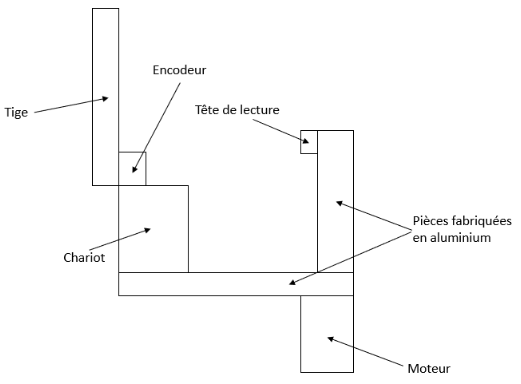
\includegraphics[width = 0.7\textwidth]{assets/figures/StructPrelim.svg}
    \caption{Structure préliminaire du système}
    \label{fig:StructPrelim}
\end{figure}